\section{Results}\label{sec:results}

\subsection{Frozen features versus end-to-end training}\label{sec:exp-main}

\begin{table}[t]
\caption{VertiBench Satellite (16 parties, 4 classes, official test set of 785 samples). Upload: payload per training sample over the 16 parties (half precision; split learning: activations and gradients at every epoch). Time: minutes on one A100-40GB for the party-side work, data loading included (split learning: one training run; SimCLR: pre-training of the 16 encoders; frozen encoders: one forward pass over all training and test images of the 16 parties). Mean\,$\pm$\,sample std over 5 seeds (the test set is fixed).}\label{tab:main}
\centering\scriptsize
\setlength{\tabcolsep}{3.5pt}
\begin{tabular}{@{}lcrccr@{}}
\toprule
Method & Bands & Upload / sample & Acc. (\%) & AUC (\%) & Time\\
\midrule
\inputtab{gen/tab_main.tex}
\bottomrule
\end{tabular}
\end{table}

\paragraph{The reference is reproduced.}
Our re-implementation of the published VertiBench configuration reaches $\reproAcc\pm\reproStd$\,\% on the 13 bands after its last epoch, in line with the published $81.2\pm0.4$\,\% (picking the best epoch on the test set would give \reproBest\,\%). Our own split-learning recipe is weaker from scratch ($77.8$\,\% on 13 bands, $77.7$\,\% on RGB) and reaches \splitPTAcc\,\% with ImageNet-initialised bottoms on RGB; the SimCLR variant of FedOnce reaches $78.5$\,\% (13 bands) and $77.6$\,\% (RGB). For these trained-from-scratch baselines the ten extra bands change accuracy by less than one point (AUC: $+1.4$ for SplitNN).

\paragraph{One upload of frozen RGB features.}
With RGB input, no party-side training and a single upload, frozen DINOv2 ViT-g/14 reaches $84.2$\,\% at 224\,px and CLIP ViT-L/14 $85.2$\,\%. The difference between two independent accuracies on 785 samples has a 95\,\% interval of about $\pm3.9$ points: against the reproduced SplitNN, CLIP's $+4.2$ points are at the edge of significance and DINOv2-g's $+3.2$ are not, whereas both are clearly above our other baselines. ~PRETRAINING-SENTENCE~ The costs differ in nature: the reproduced SplitNN exchanges activations and gradients at every one of its 50 epochs (1.56\,MiB per training sample) and needs \reproMin{} A100-minutes per training run, to be paid again for every re-training; the frozen encoders need one forward pass of every image (\timeG{} A100-minutes for DINOv2-g over all parties, training and test images, \timeClip{} for CLIP), one upload of 32--48\,KiB per sample, and a head that trains in seconds. At equal input (RGB), the encoder pass costs about as much as one run of our faster split-learning recipe (\splitRGBMin{} minutes), but only once.

\paragraph{A geographic task.}
A random forest on the recovered coordinates reaches \locRFofficial\,\% on the official split, more than any image model: the provider label of VertiBench is largely a location label, and Table~\ref{tab:main} partly ranks how well each method recognises the region. The next section separates the two.

\subsection{Why does CLIP beat DINOv2? Resolution and geography}\label{sec:exp-why}

\begin{table}[t]
\caption{Frozen encoders on VertiBench: official split (5 seeds), nearest-neighbour geolocation of the test samples from their features (median error and share within 100\,km), and five-fold cross-validation of the pooled samples with recovered coordinates, random vs.\ spatial (test set changes with the fold). Accuracy and macro AUC in \%, mean\,$\pm$\,sample std.}\label{tab:encoders}
\centering\scriptsize
\setlength{\tabcolsep}{2.4pt}
\begin{tabular}{@{}lcrrcccc@{}}
\toprule
 & Official & \multicolumn{2}{c}{Geolocation} & \multicolumn{2}{c}{Random 5-fold CV} & \multicolumn{2}{c}{Spatial 5-fold CV}\\
\cmidrule(lr){3-4}\cmidrule(lr){5-6}\cmidrule(lr){7-8}
Encoder & Acc. & km & $<$100\,km & Acc. & AUC & Acc. & AUC\\
\midrule
\inputtab{gen/tab_encoders.tex}
\bottomrule
\end{tabular}
\end{table}

Table~\ref{tab:encoders} tests three explanations of the CLIP--DINOv2 gap observed in our first extraction (85.2 vs.\ 82.6\,\%).

\paragraph{Input resolution explains most of it.}
That extraction fed DINOv2 $168$-px images ($12\times12$ patches) and CLIP $224$-px images. At 224\,px, DINOv2-g gains 1.6 points ($84.2$\,\%; paired difference \pairGsvGlDiff{} points, McNemar $p=\pairGsvGlP$), whereas CLIP loses only 0.3 points at 168\,px; the remaining gap to CLIP is 1.0 point on the official split (paired: \pairCvGlDiff{} points, 95\,\% bootstrap interval [\pairCvGlLo, \pairCvGlHi], $p=\pairCvGlP$) and 0.1 point under random cross-validation. Concatenating the mean patch token to the class token adds 0.5 points. Resizing choices matter for remote-sensing benchmarks~\cite{corley2024resizing}, and they matter here more than the choice between the two best encoders. Image--text pre-training alone is not the answer either: SigLIP-B/16 ($81.6$\,\%) is below CLIP-B/16 ($84.4$\,\%).

\paragraph{The features know where the images were taken.}
Predicting the location of a test sample by that of its nearest training sample in feature space gives a median error of 569\,km with CLIP-L, 808\,km with DINOv2-g at 224\,px and 4{,}032\,km with random weights. Across the nine encoders, accuracy on the official split follows this geolocation ability almost monotonically (Spearman $\rho=\geoSpearman$), as expected for a geographic label, and CLIP features geolocate best, consistently with the strength of CLIP-based image geolocators~\cite{haas2023streetclip,haas2024pigeon,vivanco2023geoclip}.

\paragraph{But they also carry more than location.}
Under random cross-validation of the pooled samples, coordinates alone reach $91.4$\,\%, above every encoder ($75.8$--$86.0$\,\%). Under spatial cross-validation they fall to the level of the training majority class ($61.1$ vs.\ $60.6$\,\%, AUC $58.4$), whereas the frozen features keep $69$--$74$\,\% accuracy and $73$--$77$\,\% AUC (random weights: $63.6$\,\% and $64.0$). The spread across spatial folds is large (the majority class covers 44--88\,\% of a test fold), but within folds the ranking is stable: CLIP-L stays ahead of DINOv2-g at 224\,px ($+1.7$ points on all five folds, $+2.1$ AUC on three), so its small advantage is not only region recognition. The absolute accuracies of Table~\ref{tab:main}, however, overstate what any of these models would achieve in a new region by more than 10 points.

\subsection{How little needs to be sent?}\label{sec:exp-pareto}

\begin{figure}[t]
\centering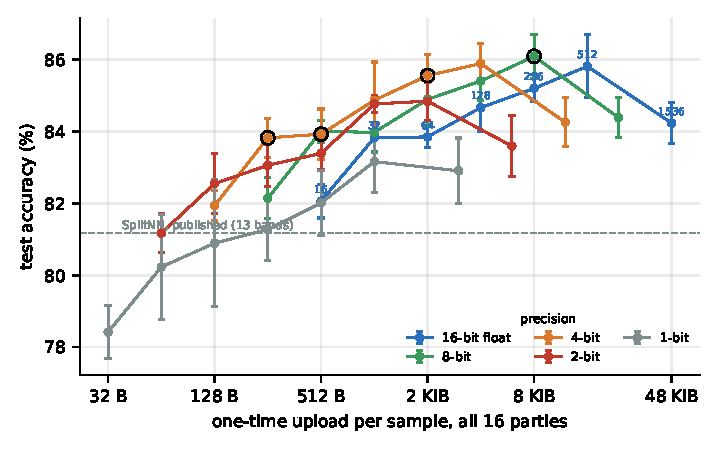
\includegraphics[width=0.78\linewidth]{gen/fig_pareto.pdf}
\caption{Accuracy versus one-time upload (bytes per sample, 16 parties) for per-party PCA (number of components $d'$ annotated on the 16-bit curve) and uniform scalar quantisation of frozen DINOv2-g features (168\,px), MLP head, mean\,$\pm$\,sample std over 5 seeds. Circles: configuration with the best \emph{validation} accuracy under a budget of 256\,B, 512\,B, 2\,KiB and 48\,KiB.}\label{fig:pareto}
\end{figure}

~TEXT-PARETO~

\subsection{Fewer parties, missing parties}\label{sec:exp-parties}

\begin{figure}[t]
\centering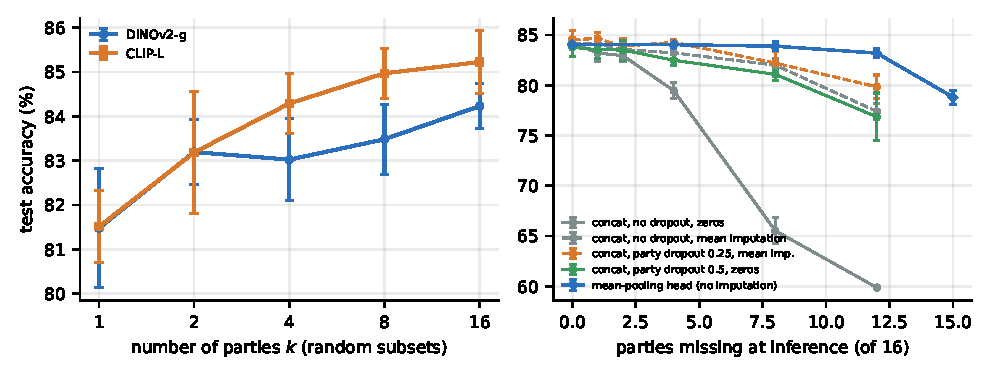
\includegraphics[width=\linewidth]{gen/fig_parties.pdf}
\caption{Left: accuracy with $k$ randomly chosen parties (3 subsets $\times$ 5 seeds). Right: parties missing at inference, replaced by zeros or by the training mean of the party, for heads trained with and without party-level dropout (5 seeds; DINOv2-g, 168\,px).}\label{fig:parties}
\end{figure}

~TEXT-PARTIES~

\subsection{What does the upload leak?}\label{sec:exp-privacy}

\begin{figure}[t]
\centering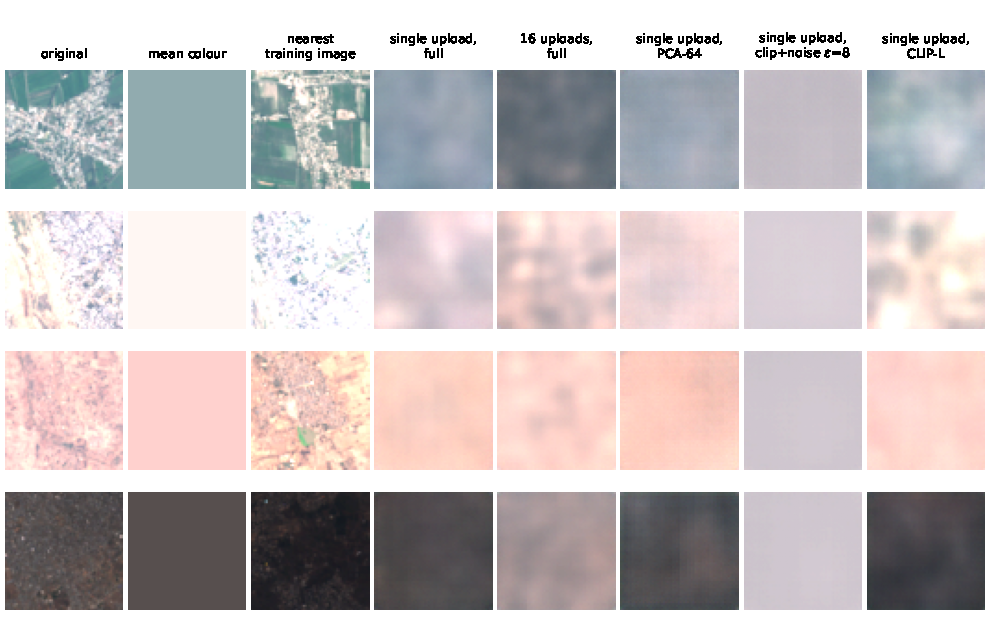
\includegraphics[width=\linewidth]{gen/fig_inversion.pdf}
\caption{Inversion attack on held-out test images ($64\times64$ RGB thumbnails of four test locations, party 0; brightness $\times3$ for display, identical for all panels). From left to right: original; its mean colour; nearest training image in DINOv2-g feature space; decoder output from one full DINOv2-g upload, from the 16 uploads of the location, from a PCA-64 upload, from a clipped noisy upload ($\varepsilon=8$), and from one CLIP-L upload.}\label{fig:inversion}
\end{figure}

\begin{table}[t]
\caption{Utility versus leakage of the upload format (16 parties, 168-px DINOv2-g unless stated). Upload: bytes per sample; accuracy on the VertiBench test set (5 seeds); PSNR (3 decoder seeds for the full, PCA-64 and $\varepsilon=8$ rows) and SSIM of the single-upload attack; Re-id: share of test images whose reconstruction is closer to them than to any other of the 12.5k test images (chance: 0.01\,\%); Joint: PSNR of the attack that sees the 16 uploads of a location. Clip + noise: the Gaussian mechanism of Sec.~\ref{sec:method}, per-upload $(\varepsilon, 10^{-5})$.}\label{tab:privacy}
\centering\scriptsize
\setlength{\tabcolsep}{3.5pt}
\begin{tabular}{@{}lrccccc@{}}
\toprule
Upload format & Upload & Acc. (\%) & PSNR (dB) & SSIM & Re-id (\%) & Joint (dB)\\
\midrule
\inputtab{gen/tab_privacy.tex}
\bottomrule
\end{tabular}
\end{table}

~TEXT-PRIVACY~

\subsection{WorldStrat: two sensors, and what a random split hides}\label{sec:exp-ws}

\begin{table}[t]
\caption{WorldStrat, IPCC land cover (7 classes, 3{,}925 locations). Frozen DINOv2 ViT-g/14 features, MLP head. Five-fold cross-validation with random or spatial folds (each fold is the test set once). Accuracy and macro AUC in \%, mean\,$\pm$\,sample std over folds.}\label{tab:ws}
\centering\scriptsize
\setlength{\tabcolsep}{4pt}
\begin{tabular}{@{}lcccc@{}}
\toprule
 & \multicolumn{2}{c}{Random 5-fold CV} & \multicolumn{2}{c}{Spatial 5-fold CV}\\
\cmidrule(lr){2-3}\cmidrule(lr){4-5}
Inputs & Acc. & AUC & Acc. & AUC\\
\midrule
\inputtab{gen/tab_ws_ipcc.tex}
\bottomrule
\end{tabular}
\end{table}

~TEXT-WS~
